\begin{frame}
	\frametitle{Was steckt hinter der Abstraktion ``Computer''?}

	\begin{itemize}
		\item Das ist natürlich etwas umfangreicher,
		\item daher werden wir uns morgen damit ausführlich beschäftigen.
		\item Aber jetzt wir wollen uns einmal ansehen, \ldots
	\end{itemize}

\end{frame}


\sectionFrame{
%Vom Sandkorn zum Chip\\
%oder:\\
 Woraus besteht eigentlich\\
 ein Computerchip?}{}

\begin{frame}
	\frametitle{``All computers are just carefully organized sand''}
	\begin{figure}
		\centering
		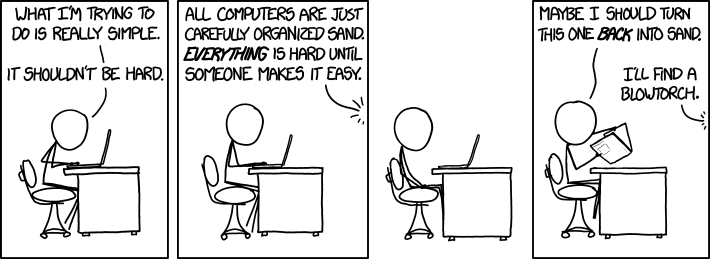
\includegraphics[width=.8\textwidth]{images/shouldnt_be_hard.png}
		\caption{``Shouldn't Be Hard'' by Randall Munroe
		CC-BY-NC-2.5, \url{http://xkcd.com/1349}}
	\end{figure}

	\begin{quote}<2->
		(six hours later) ARGH. How are these stupid microchips so durable?!
		All I want is to undo a massive industrial process with household
		tools!
	\end{quote}
\end{frame}

\begin{frame}
	\frametitle{``All computers are just carefully organized sand''}

	\begin{figure}
		\centering
		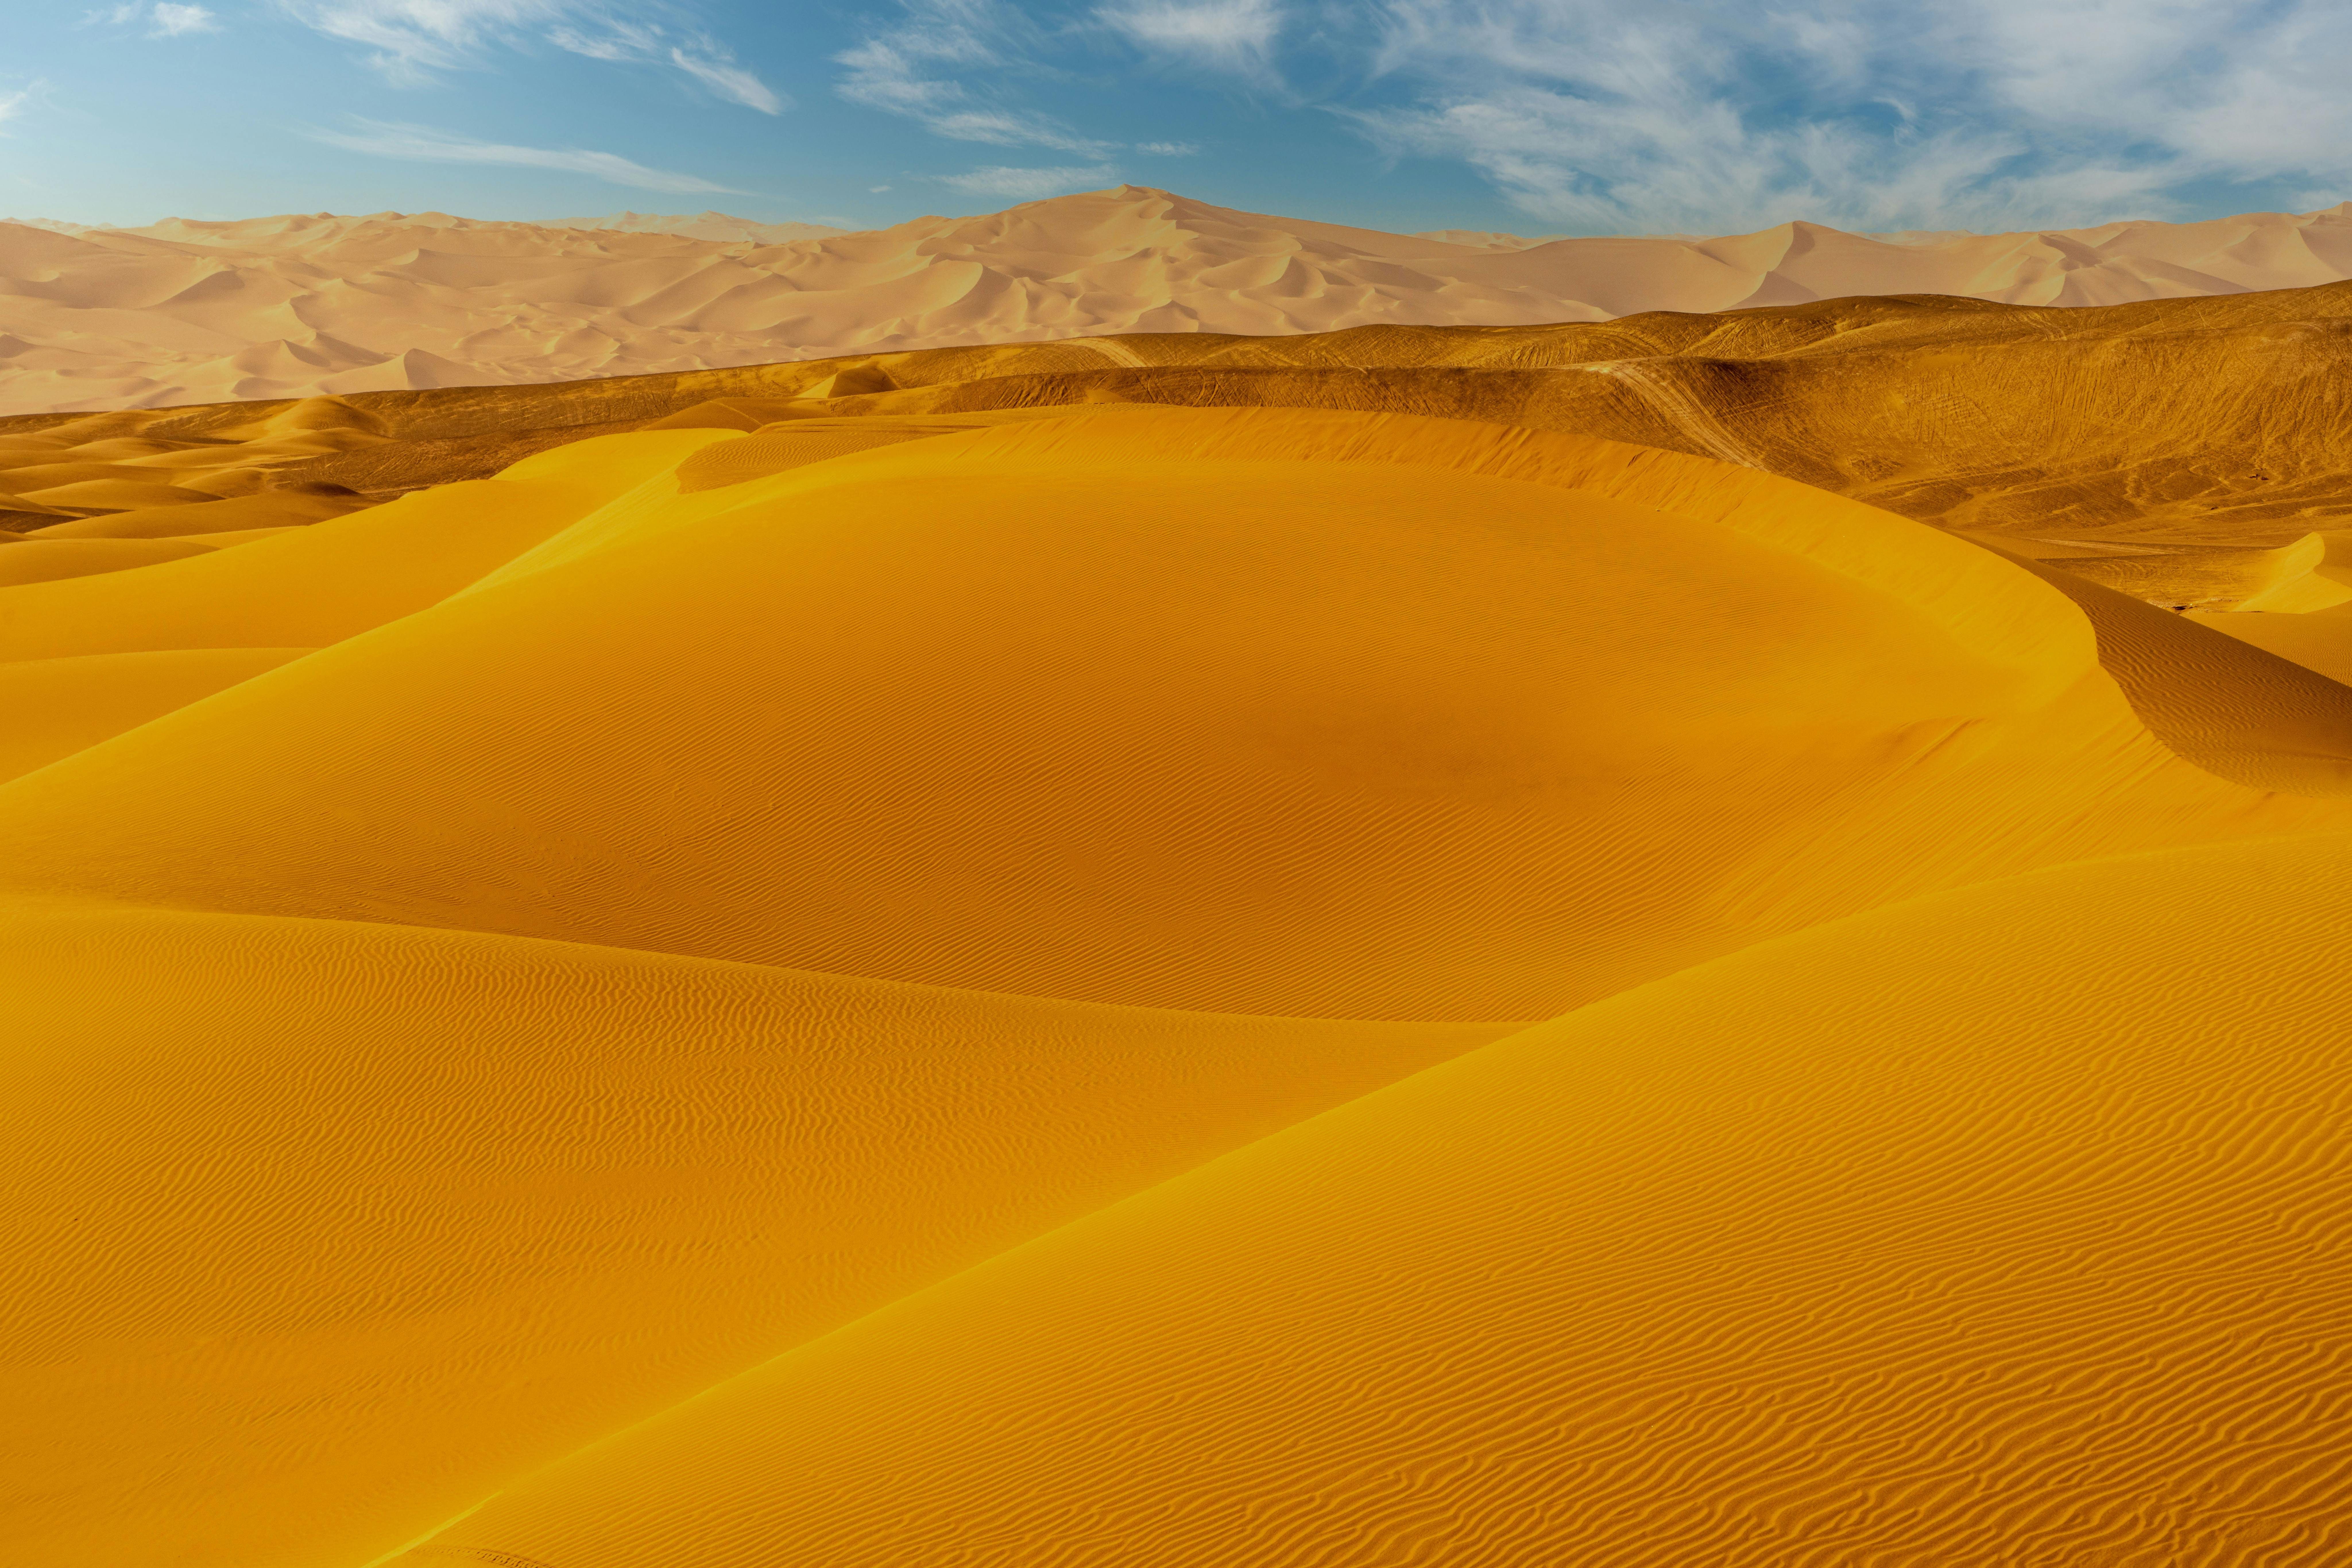
\includegraphics[width=.7\textwidth]{images/the_desert.jpg}
		\caption{``Siliziumquelle'' SiO\textsubscript{2} \\
		``The Desert'' by John O'Nolan
		CC-BY-2.0, \url{http://flic.kr/p/aEJ8Rk}}
	\end{figure}
\end{frame}

\begin{frame}
	\frametitle{Vom Sandkorn zum Chip}
	\begin{columns}[onlytextwidth]
		\begin{column}{0.6\textwidth}
			\begin{figure}
				\centering
				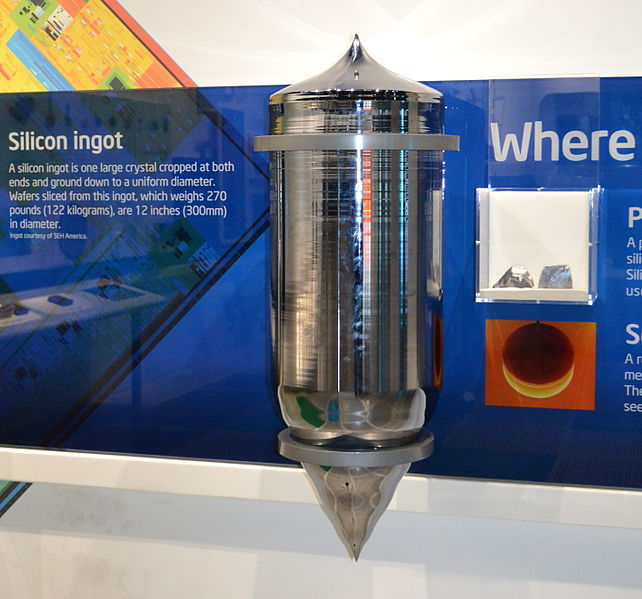
\includegraphics[width=.6\textwidth]{images/Siligon_ingot_at_Intel_Museum.JPG}

				\caption{Hochreiner Silizium-Einkristall.\\
					By Oleg Alexandrov CC-BY-SA-3.0\\
					via Wikimedia Commons.}
			\end{figure}
		\end{column}
		\begin{column}{0.45\textwidth}
			\begin{itemize}
				\item Durchmesser 30--\SI{40}{\centi\meter}
				\item Länge \SI{2}{\meter}
				\item Gewicht \SI{> 100}{\kilo\gram}
				\item Reinheitsgrad \SI{>99.9999999}{\percent}
			\end{itemize}
		\end{column}
	\end{columns}
\end{frame}

\begin{frame}
	\begin{columns}
		\begin{column}{.5\textwidth}
			\begin{figure}
				\centering
				\includegraphics[width=.85\textwidth]{images/Wafer_intel.jpg}
				\caption{Ein Wafer \textcopyright{} Intel}
			\end{figure}
		\end{column}
		\begin{column}{.5\textwidth}
			\begin{figure}
				\centering
				\includegraphics[width=.9\textwidth]{images/TTPchip.png}
				\caption{Chip im Package}
			\end{figure}
		\end{column}
	\end{columns}
\end{frame}

\begin{frame}
% good slides from intel at http://download.intel.com/newsroom/kits/chipmaking/pdfs/Sand-to-Silicon_32nm-Version.pdf
	\begin{figure}
		\centering
		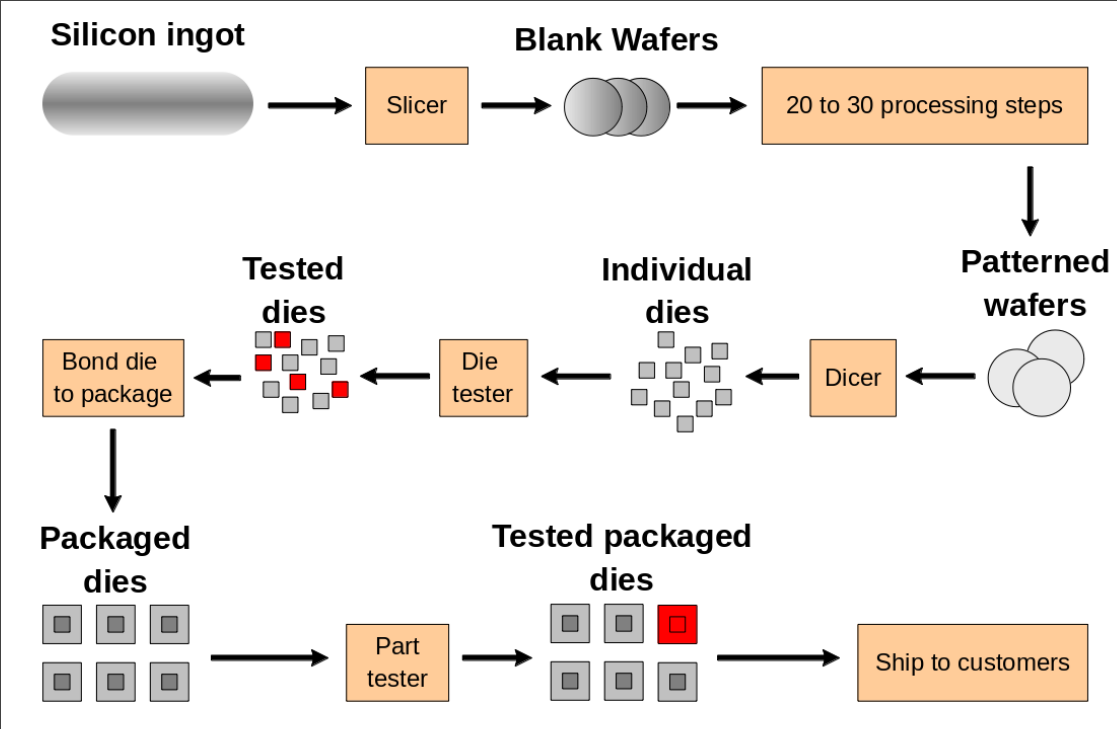
\includegraphics[width=.8\textwidth]{images/chip_fertigung.png}
		\vspace{0.3cm}
		\caption{Industrielle Chipfertigung}
	\end{figure}

\end{frame}


\begin{frame}
	\frametitle{Vom Transistor zum Mikroprozessor}
	\begin{block}{Was macht man nun mit den ganzen Transistoren?}
		\begin{itemize}
			\item Standard Cell Designer entwerfen logische Grundbausteine
				(AND, OR, NAND, \ldots) aus Transistoren in konkreter
				Technologie, z.B.\ \SI{14}{\nano\meter}.
			\item Bibliothek von solchen ``Standard Cells'' mit
				unterschiedlichen Vor-/Nachteilen: Geschwindigkeit, Größe,
				Stromverbrauch, \ldots
		\end{itemize}
	\end{block}
\end{frame}

\begin{frame}
	\begin{block}{Was macht man mit den Standard Cells?}
		\begin{itemize}
			\item Designer benutzen Standard Cell Bibliothek um Funktionsblock
				nach ihren Vorstellungen zu realisieren.
			\item Hier gibt es viel Tool-Support.
			\item Schaltungsdesigner arbeiten meist mit ``Beschreibungssprachen'',
                              ähnlich wie Programmierer.
			\item Ein komplexer Chip kann hunderte Millionen Transistoren
				beinhalten.
		\end{itemize}
	\end{block}
\end{frame}

\sectionFrame{Grenzen der Chiptechnologie}{}


\begin{frame}
	\frametitle{Chiptechnologie --- ein Größenvergleich}
	\begin{exampleblock}{Stellen Sie sich vor:}
		Ein \SI{14}{\nano\meter} Transistor % 0.058um^2
		wäre so groß wie ein Fingernagel % ~ 1 cm^2 = 10^8 um^2
                % wäre so groß wie eine Hand % 0.054 m^2 = 5.4*10^10 um^2
		\ldots\\

		\pause

		\bigskip
		\ldots dann wäre ein menschliches Haar % d ~ 100um => A ~ 7854 um^2
                so dick dass es auf dem Podium keinen Platz mehr hätte. % d ~ 3m => A < 13.36 m^2

	\end{exampleblock}

\end{frame}

\begin{frame}
	\frametitle{Chiptechnologie --- ein Größenvergleich}
	\begin{exampleblock}{Anders gesagt:}
		Ein rotes Blutkörperchen ist etwa 500x größer als ein \SI{14}{\nano\meter} Transistor!

		% kleinste RBK  d ~ 6 um => A ~ 28.27 um^2
	\end{exampleblock}
\end{frame}

\begin{frame}
	\frametitle{Chiptechnologie --- ein Generationenvergleich}
	\begin{columns}[t]
		\begin{column}{.45\textwidth}
			\begin{block}{Intel 4004}
				\begin{itemize}
					\item Einführung 1971
					\item 4-Bit (vier!) Architektur
					\item 1 Kern
					\item \SI{740}{\kilo\hertz}
					\item 2300 Transistoren
					\item 16 Pins
					\item \SI{144}{\milli\meter\squared} Die Fläche
					\item \SI{10}{\micro\meter} Prozess
				\end{itemize}
			\end{block}
		\end{column}
		\begin{column}{.55\textwidth}
			\begin{block}{Intel Core i7 4770 (Haswell)}
				\begin{itemize}
					\item Einführung 2013
					\item 64-Bit Architektur
					\item 4 Kerne
					\item \SI{3.4}{\giga\hertz}
					\item 1.4 Milliarden Transistoren
					\item 1150 Pins
					\item \SI{177}{\milli\meter\squared} Die Fläche
					\item \SI{22}{\nano\meter} Prozess
				\end{itemize}
			\end{block}
		\end{column}
	\end{columns}
\end{frame}

\begin{frame}
	\frametitle{Chiptechnologie --- ein Generationenvergleich}
	\only<1>{
		\begin{figure}
			\centering
			\includegraphics[width=.4\textwidth]{images/chip_4004-i7_then.png}
			\vspace{0.5cm}
			\caption{Die Designs in ihrer Technologie gefertigt \textcopyright{} Intel}
		\end{figure}
	}
	\only<2-3>{
		\begin{figure}
			\centering
			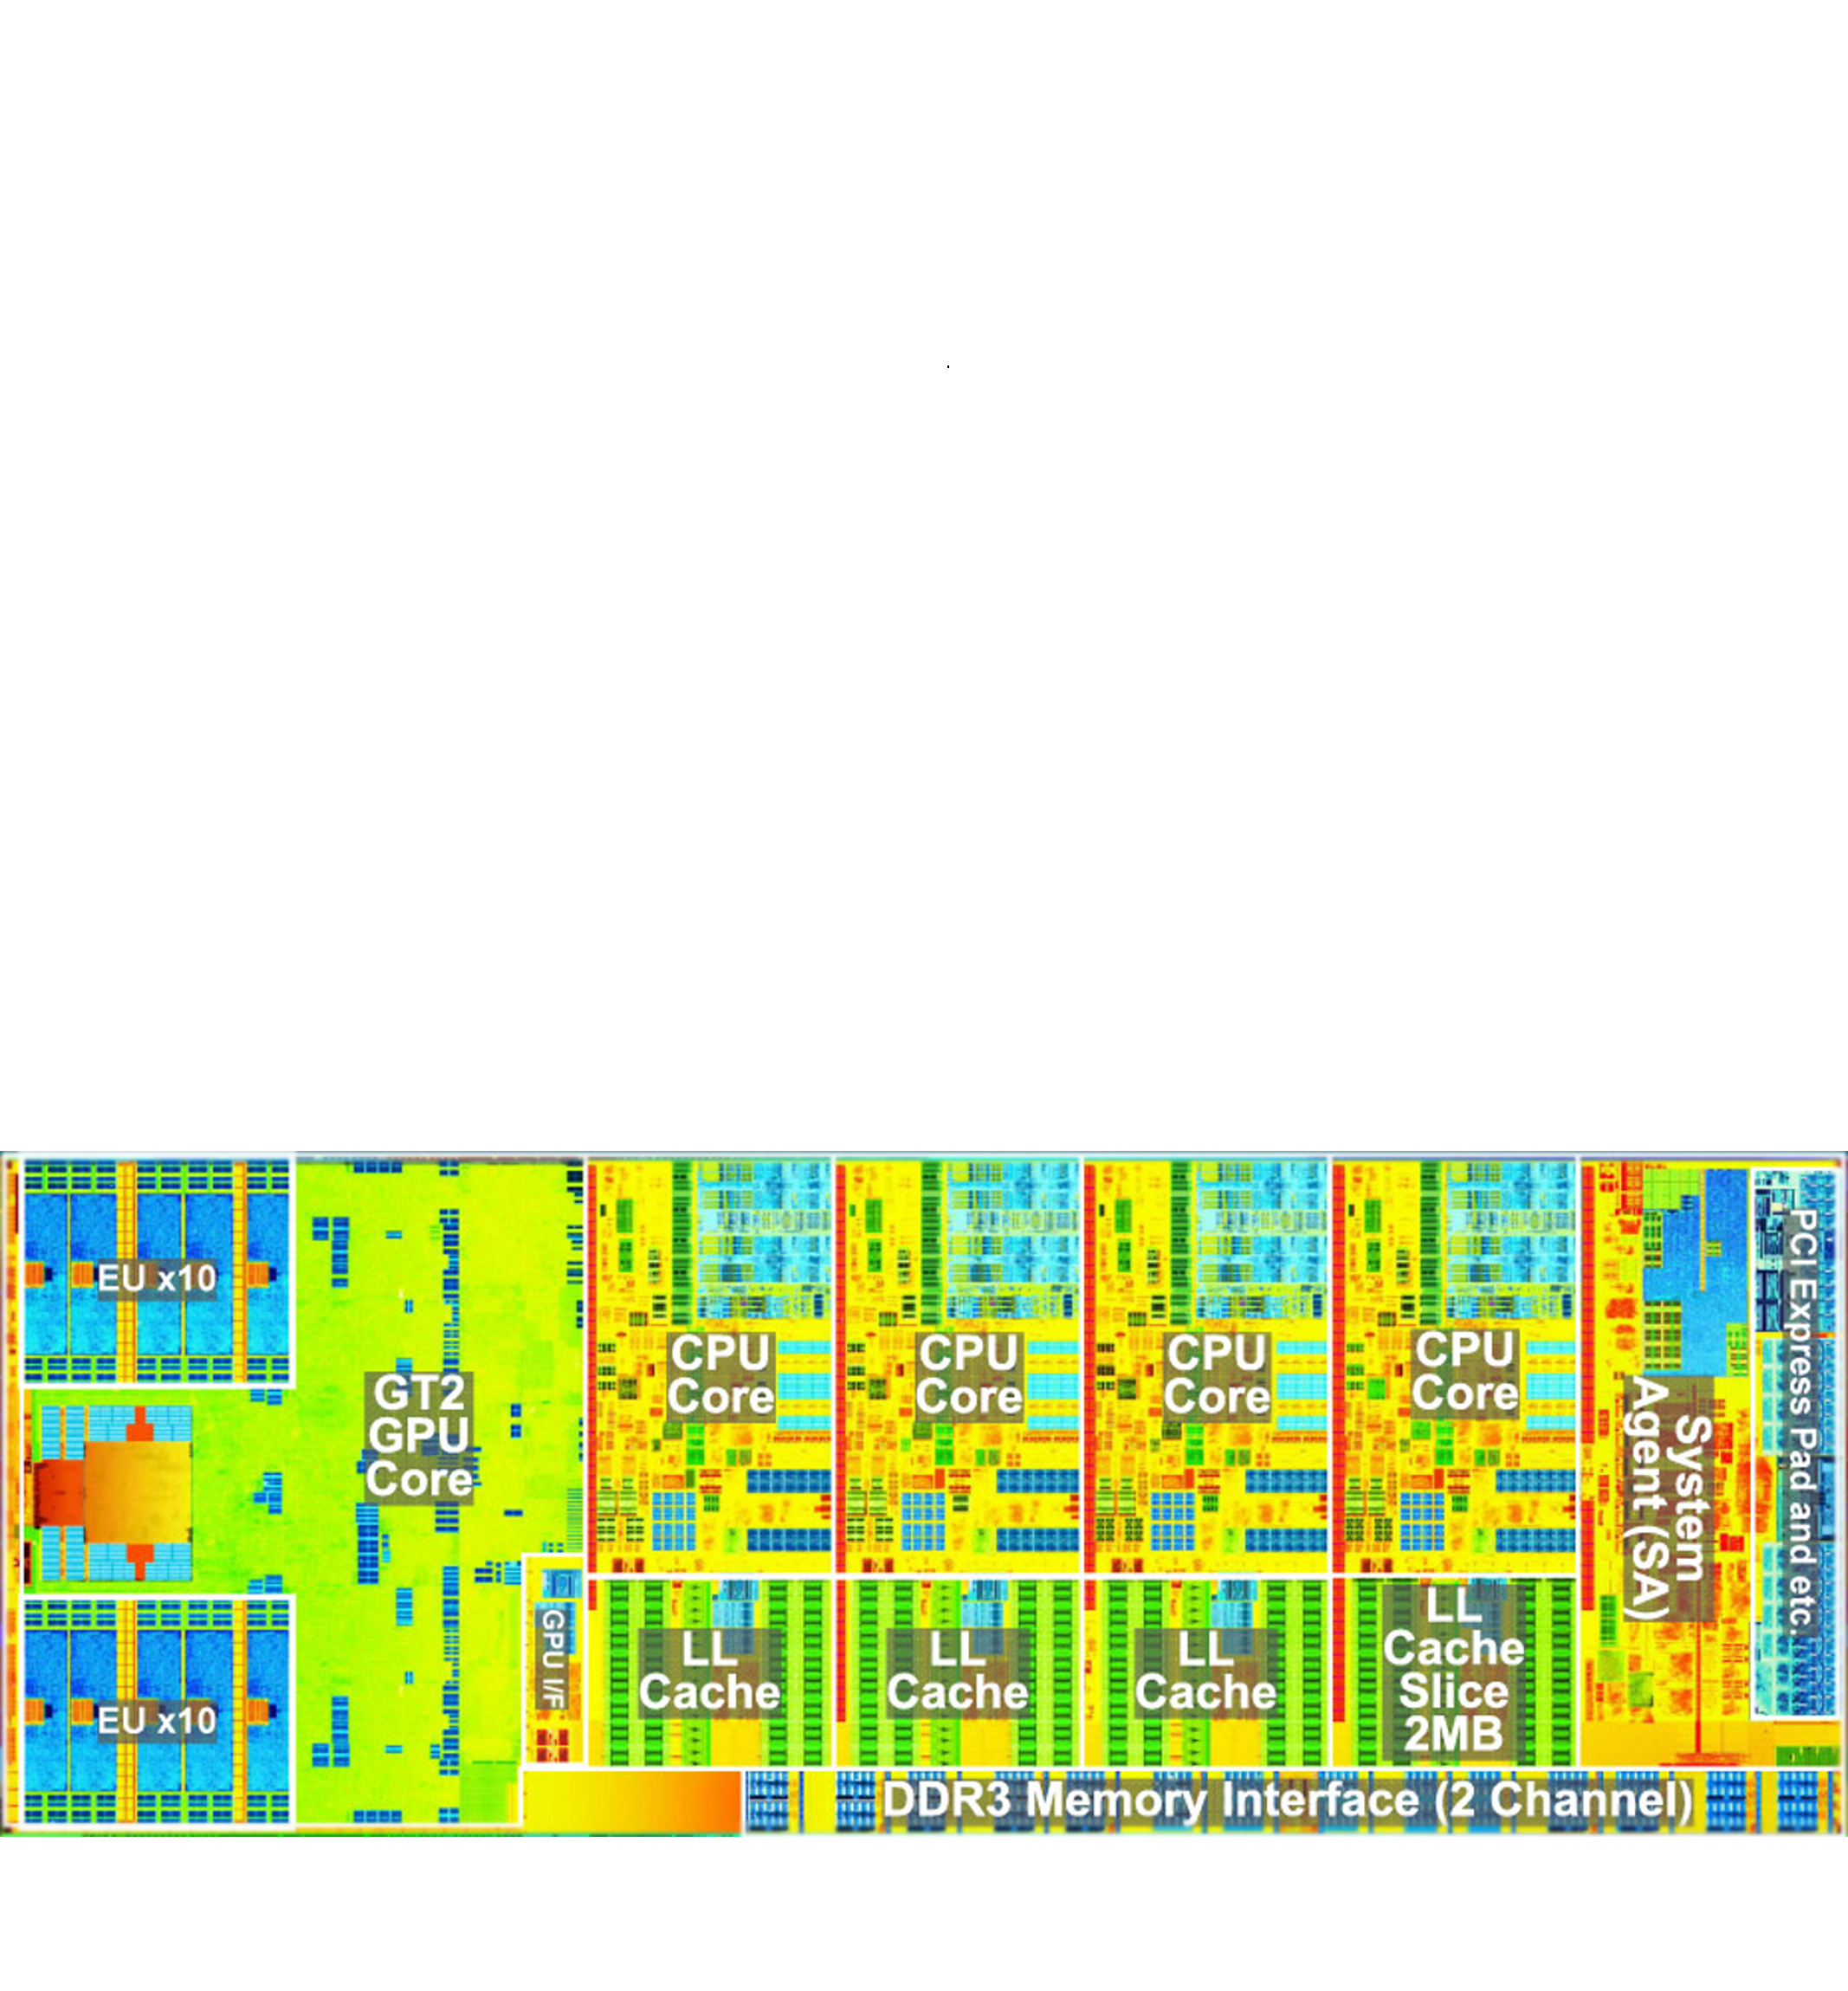
\includegraphics[width=.4\textwidth]{images/chip_4004-i7_now.png}
			\vspace{0.5cm}
			\caption{Das 40 Jahre altes Design in aktueller Technologie
				gefertigt \textcopyright{} Intel}
		\end{figure}
	}
	\begin{tikzpicture}[overlay,remember picture]
		\node[right] (i7)   at (0.7,3.7) {2013: Intel i7};
		\node<1>[below right] (four) at (0.7,7.15) {1971: Intel 4004};
		\node<2-3>[below right,align=left] (four2_2) at (0.7,7.15) {\alert{2013}: Intel 4004\\
			\SI{144}{\milli\meter\squared} $\Rightarrow$ \SI{0.0003}{\milli\meter\squared}};
		\draw<3>[latex-, red] (7.1,6.925) -- +(0.75,0.75);
	\end{tikzpicture}
\end{frame}

\begin{frame}
	\frametitle{Chiptechnologie --- Miniaturisierung}
	\only<1>{
		\begin{figure}
			\centering
			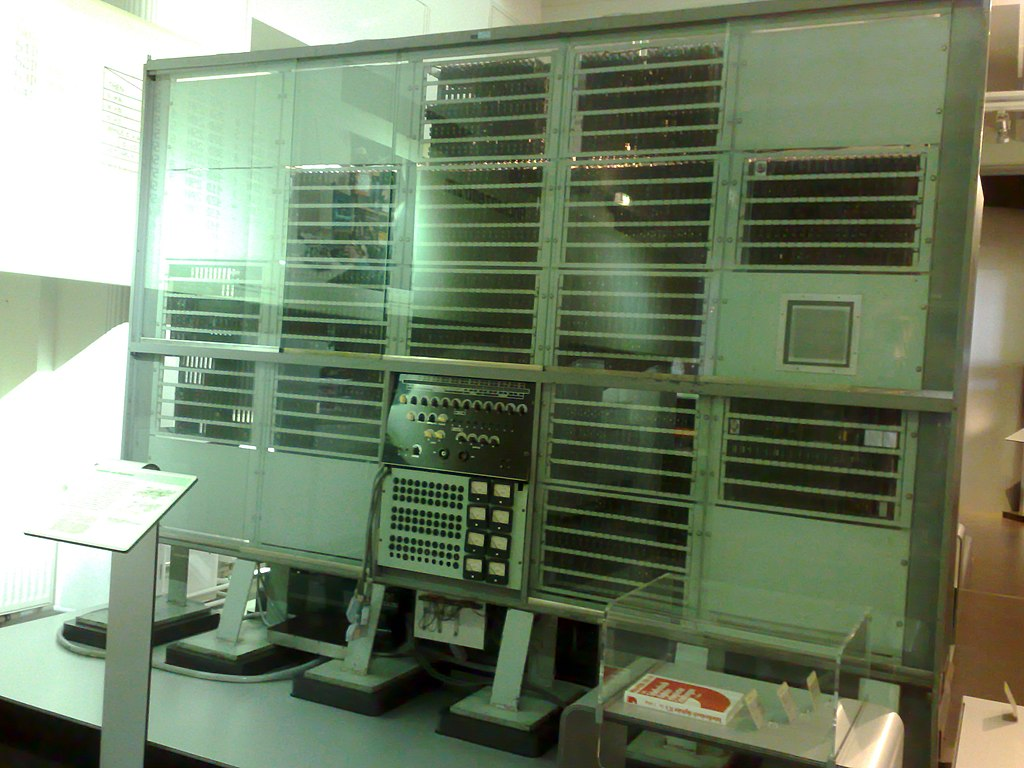
\includegraphics[height=.7\textheight]{images/Mailuefterl.jpg}
			\caption{Mailüfterl (1958); 8000 ``Transistoren'',
				\SI{20}{\kilo\meter} Schaltdraht\\
				By Florian Staudacher CC-BY-3.0 via Wikimedia Commons.}
		\end{figure}
	}
	\only<2>{
		\begin{figure}
			\centering
			\includegraphics[height=.7\textheight]{images/trans_trad.png}
			\caption{Traditionalles FET-Transistordesign \textcopyright{} Intel}
		\end{figure}
	}
	\only<3>{
		\begin{figure}
			\centering
			\includegraphics[height=.7\textheight]{images/trans_14nm.png}
			\caption{\SI{14}{\nano\meter} FinFET-Transistordesign \textcopyright{} Intel}
		\end{figure}
	}
	\only<4>{
		\begin{figure}
			\centering
			\includegraphics[height=.7\textheight]{images/14nm_fin.png}
			\caption{\SI{14}{\nano\meter} FinFET-Transistor Querschnitt \textcopyright{} Intel}
		\end{figure}
	}
	\only<5>{
		\begin{figure}
			\centering
			\includegraphics[height=.7\textheight]{images/14nm_full.png}
			\caption{\SI{14}{\nano\meter} FinFET-Transistor Querschnitt \textcopyright{} Intel}
		\end{figure}
	}
	\only<6>{
		\begin{figure}
			\centering
			\includegraphics[height=.7\textheight]{images/14nm_die.png}
			\caption{\SI{14}{\nano\meter} FinFET-Transistor im Chip \textcopyright{} Intel}
		\end{figure}
	}

\end{frame}

\begin{frame}
	\frametitle{Grenzen der Chiptechnologie}
	\begin{alertblock}{Wo ist der \SI[detect-weight]{30}{\giga\hertz} Prozessor?}

		Oder: Warum stagnieren in letzter Zeit die Taktraten?

	\end{alertblock}
\end{frame}

\begin{frame}
	\frametitle{Grenzen der Chiptechnologie}

	\begin{block}{Bestimmt nicht einfach nur der Taktgeber die Taktrate?}
		\begin{itemize}
			\item Wer bestimmt eigentlich, mit welcher Taktrate mein Rechner läuft?
			\item Wieso holen Übertakter noch enorme Steigerungen raus?
		\end{itemize}
	\end{block}

	\begin{exampleblock}{Probieren wir es aus!}<2->
		Bauen wir eine Schaltung ohne Taktgeber und beobachten, was passiert.
	\end{exampleblock}
\end{frame}


\begin{frame}
	\frametitle{Wir bauen einen ``Ringoszillator'' --- Aufbau}

	\begin{block}{Ringoszillator}
		\begin{center}
			\begin{tikzpicture}[circuit logic US]
				\tikzstyle{branch}=[fill,shape=circle,minimum size=3pt,inner sep=0pt]

				\coordinate (ports) at (-2,0);

				\node [buffer gate] (b1) at (1,0) {};
				\node [buffer gate] (b2) at (2,0) {};
				\node [buffer gate] (b3) at (3,0) {};

				\node [buffer gate] (b4) at (4.5,0) {};

				\node [not gate] (n1) at (5.5,0) {};

				\draw (n1.output) -- ([xshift=7]n1.output) node[branch] (branch1) {}
				-- +(0,1) node (t1) {};

				\draw (b1.input) -- ([xshift=-7]b1.input) |- (t1.center);

				\draw (b1.output) -- (b2.input);
				\draw (b2.output) -- (b3.input);

				\draw (b3.output) -- ($(b3.output) + (0.1,0)$);
				\draw[dotted] ($(b3.output) + (0.1,0)$) -- ($(b4.input) + (-0.1,0)$);
				\draw ($(b4.input) + (-0.1,0)$) -- (b4.input);

				\draw (b4.output) -- (n1.input);

				\draw[->] (branch1.center) -- +(0.75,0) node [anchor=west] {Takt};


			\end{tikzpicture}
		\end{center}

		\begin{itemize}
			\item Die Frequenz des erzeugten Taktes ist nur durch die Laufzeit
				einer langen Kette von Gattern bestimmt.
		\end{itemize}
	\end{block}
\end{frame}

\liveDemo{Wir bauen einen ``Ringoszillator''}

\begin{frame}
	\frametitle{Wir bauen einen ``Ringoszillator'' --- Erkenntnisse}

	\begin{block}{Wir haben gesehen dass:}
		\begin{itemize}
			\item \ldots die Frequenz des Ringoszillators temperaturabhängig ist!
			\item Also muss auch die Gatterlaufzeit temperaturabhängig sein!
			\item Eine konstante Taktperiode ist also wieder eine
				Abstraktion.
		\end{itemize}
	\end{block}

	\begin{block}{Warum brauchen wir diese Abstraktion?}<2->
		\begin{itemize}
			\item Die Signallaufzeiten am Chip sind abhängig von Temperatur und Spannung.
			\item Darum will sich ein Programmierer nicht kümmern müssen,
			\item daher werden diese Abhängigkeiten verborgen:
			\item Wir wählen eine konstante Taktperiode, die größer ist als die Laufzeit unter
				den schlechtesten Bedingungen.
		\end{itemize}
	\end{block}
\end{frame}

\begin{frame}
	\frametitle{Grenzen der Chiptechnologie}

	\begin{alertblock}{Aber:}
		\begin{itemize}
			\item Woher kommen diese Laufzeiten eigentlich?
			\item Sind elektrische Signale nicht unendlich schnell?
		\end{itemize}
	\end{alertblock}

\end{frame}

\begin{frame}

	\begin{block}{Grenze 1: Lichtgeschwindigkeit \phantom{/}}

		\begin{itemize}
			\item $\SI{30}{\giga\hertz} =$ \num{30e9} Taktperioden pro
				Sekunde,
			\item Lichtgeschwindigkeit 	$c_0 \approx
				\SI{3e8}{\meter\per\second}$ (im Vakuum)\\
				Signale breiten sich am Chip mit $\approx \mathsf{^2/_3}~c_0$ aus.
			\item<2-> \alert<2>{In einer Taktperiode legt das Licht also nur
					\SI{1}{\centi\meter} zurück!}
				\item<3-> Bei einem Chip mit \SI{2}{\centi\meter} Kantenlänge
					braucht das Taktsignal also mehr als 2 Takte quer durch
					den Chip.
				\item<3-> Das widerspricht der Abstraktion, dass Taktflanken
					überall am Chip ``synchron'' stattfinden.
			\end{itemize}
		\end{block}

\end{frame}



\begin{frame}

	\begin{block}{Grenze 2: Lade-/Entladevorgänge}

		\begin{itemize}
			\item Gatter sind aus Transistoren aufgebaut.
			\item Idealerweise sind Transistoren Schalter (Abstraktion \ldots)
			\item Bei genauerer Betrachtung verhalten sich Transistoren (und
				Leitungen) wie Kondensatoren und Widerstände.
			\item Laden bzw.\ Entladen von Kondensatoren über einen Widerstand
				benötigt Zeit (vgl.: über Schlauch Gefäß füllen).
				% Publikumsfrage: Warum nimmt man nicht einfach einen dickeren
				% Schlauch?
			\item Diese Zeit begrenzt die erreichbare Geschwindigkeit des
				Chips.
		\end{itemize}
	\end{block}
\end{frame}


%\begin{frame}
%
%	\begin{block}{Grenze 2: Lichtgeschwindigkeit}
%
%	\begin{itemize}
%		\item $\SI{30}{\giga\hertz} = \SI{30e9}{\per\second}$,\\
%			$c \approx \SI{3e8}{\meter\per\second}$,\\
%			Chip: ca. $\SI{1}{\centi\meter\squared}$
%		\item \num{30e9} Mal pro Sekunde \SI{1}{\centi\meter} zurücklegen:
%			$\num{30e9} \cdot \SI{1}{\centi\meter\per\second} =
%			\SI{3e8}{\meter\per\second} = c$
%		\item D.h.\ in einem \SI{30}{\giga\hertz} Prozessor müssten sich die
%			Signale im Prozessor mit Lichtgeschwindigkeit ausbreiten.
%	\end{itemize}
%\end{block}
%
%\end{frame}


%\begin{frame}
%
%	\begin{block}{Problem 3: Ladungsausbreitung}
%		\begin{itemize}
%			\item Die Bewegung/Diffusion der Ladungsträger im Prozessor ist beschränkt
%			\item Bei Silizium typischerweise mit \SI{\approx
%				0.1}{\milli\meter\per\nano\second}
%		\end{itemize}
%	\end{block}
%
%\end{frame}
%


\begin{frame}

	\begin{alertblock}{Mehr Rechenleistung bei gleicher Geschwindigkeit?}
		Kann man die Physik überlisten?
	\end{alertblock}

\end{frame}

\begin{frame}

	\begin{block}{Lösung 1: Multi-Core und vernetzte Rechner}
		\begin{itemize}
			\item Moderne Desktop Computer: \numrange{4}{16} Prozessoren
				(Cores) verbaut in einem Chip, Tendenz steigend.
			\item Moderne Grafikkarten: über 1000 ``Cores''.
			\item Parallele Programme erfordern neue Programmiertechniken; \\
				\alert{große Herausforderung für die Informatik!}
		\end{itemize}
	\end{block}

\end{frame}

\begin{frame}

	\begin{block}{Lösung 2: Spezialisiertes Design}
		\begin{itemize}
			\item Bisher betrachtet: ``general-purpose'' Prozessoren die für
				verschiedenste Einsatzbereiche geeignet sind.
			\item Programmierbarkeit und Vielseitigkeit kosten Effizienz.
			\item Spezialisierte Designs (ASICs) erreichen eine Effizienz die
				mit general-purpose Lösungen nicht erreichbar ist.
			\item Höherer Entwicklungsaufwand, aber unverzichtbar für
				Anwendungsbereiche, in denen general-purpose Lösungen die
				benötigten Anforderungen (Performance, Verlustleistung,
				Fehlertoleranz, \ldots) nicht erfüllen.
		\end{itemize}
	\end{block}

\end{frame}
